\documentclass[20pt]{article}
\usepackage[utf8]{inputenc}
\usepackage{amsmath, amssymb, amsthm}
\usepackage{titlesec}
\usepackage{graphicx}
\usepackage{chngcntr}
\usepackage{tikz}
\usepackage{pgfplots}
% Customization -------

% Paper size, margin
\usepackage[letterpaper,top=1.5cm,bottom=1.5cm,left=1.75cm,right=1.75cm,heightrounded]{geometry}

% line height
\renewcommand{\baselinestretch}{1.15} % line space

% Paragraph indentation 
\setlength{\parindent}{0pt} % no indent
\graphicspath{ {./images/} }

% Paragraph spacing
\setlength{\parskip}{0.8em} % space between paragraphs

% Section number formatting
\titleformat{\section}[hang]{\bfseries}{Problem \thesection\ }{0pt}{}

% --------------------

\title{Homework 04}
\author{Farbod Mohammadzadeh\\1008360462}
\date{25 Novermber 2023}

\begin{document}
\Large
\maketitle

\newpage

\section*{Part A:}

The continuous-time equations of motion for a unit mass subject to a piecewise constant force \(f(t) = p_n\) over intervals of length 1 second are given by:

\[
    m \cdot x''(t) = f(t)
\]

Substituting \(m = 1\) (unit mass), integrating once to find velocity, and then integrating again to find position, we get:

\[
    x'(t) = \int f(t) \, dt = p_n
\]

\[
    x(t) = \int x'(t) \, dt = \int p_n \, dt = p_n \cdot t + C
\]

Applying the initial conditions \(x(0) = 0\) and \(x'(0) = 0\), we find \(C = 0\), so:

\[
    x(t) = \sum_{k=1}^n p_k \cdot t
\]

Now, discretizing this system over intervals of 1 second and evaluating at \(t = n\), we get the discrete-time equations:

\[
    x(n) = x(n-1) + \sum_{k=n-1}^n p_k
\]

\[
    x'(n) = p_n
\]

These are consistent with the provided state-space equations:

\[
    \begin{bmatrix}
        x(n) \\
        x'(n)
    \end{bmatrix}
    =
    \begin{bmatrix}
        1 & 1 \\
        0 & 1
    \end{bmatrix}
    \begin{bmatrix}
        x(n-1) \\
        x'(n-1)
    \end{bmatrix}
    +
    \begin{bmatrix}
        \frac{1}{2} \\
        1
    \end{bmatrix}
    p_n
\]

\newpage

\section*{Part B:}


The optimization problem is to minimize the objective function

\[
    \sum_{n=1}^{10} (p_n)^2
\]

subject to the constraints \(x(10) = 1\) and \(x'(10) = 0\). We can formulate this problem using the method of Lagrange multipliers. The Lagrangian is given by

\[
    L(p, \lambda_1, \lambda_2) = \sum_{n=1}^{10} (p_n)^2 + \lambda_1 \cdot (x(10) - 1) + \lambda_2 \cdot x'(10)
\]

where \(\lambda_1\) and \(\lambda_2\) are the Lagrange multipliers. The necessary conditions for optimality are obtained by taking partial derivatives and setting them equal to zero:

\[
    \begin{aligned}
         & \frac{\partial L}{\partial p_n} = 2p_n + \lambda_1 = 0, \quad \text{for } n = 1, 2, \ldots, 10 \\
         & \frac{\partial L}{\partial \lambda_1} = x(10) - 1 = 0                                          \\
         & \frac{\partial L}{\partial \lambda_2} = x'(10) = 0
    \end{aligned}
\]

Solving this system of equations will yield the optimal values for \(p_n\). Once we have these optimal values, we can use them to simulate the system and plot the optimal control input \(f(t)\), resulting position \(x(t)\), and velocity \(x'(t)\).
 
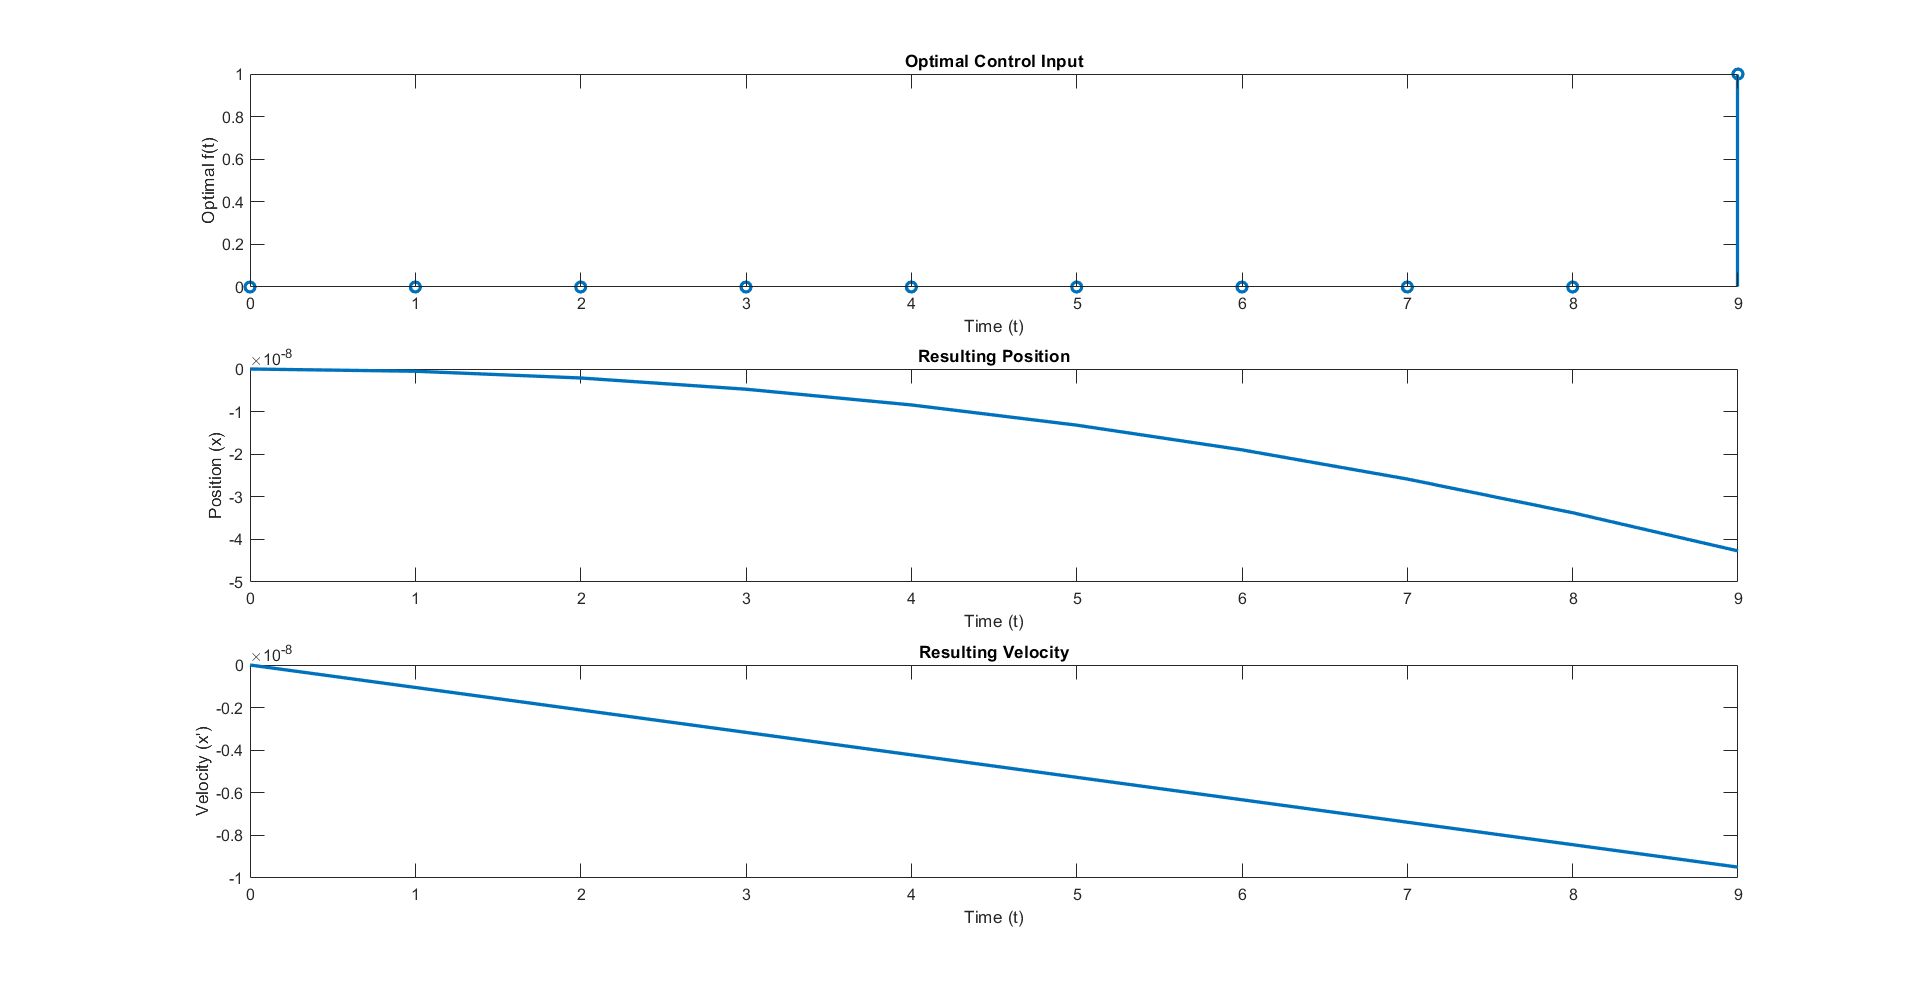
\includegraphics[width=\textwidth]{partB.png}



\end{document}